\documentclass[11pt,a4paper]{article}
\usepackage[left=2cm, text={17cm,24cm}, top=3cm]{geometry}
\usepackage[czech]{babel}
\usepackage[utf8]{inputenc}
\usepackage{times}
\usepackage[unicode]{hyperref} %pro křížové odkazy
\usepackage{graphicx} %pro práci s obrázky
\usepackage{amsmath} %sazba matematiky
\usepackage{xcolor} %barvičky
\usepackage{listings} %algoritmy, sazba kódu
\usepackage{algpseudocode}
\usepackage{pxfonts}

\lstset{
  language=C,
  numbersep=5pt,
  breaklines=true,  
  breakatwhitespace=false,
  basicstyle=\ttfamily,
  commentstyle=\color{gray},
  keywordstyle=\bfseries,
  showstringspaces=false,
  %numbers=left,
  %numberstyle=\tiny\color{gray},
}

\title{Documentation for IFJ \& IAL project}
\author{Michal Šmahel}
\date{September 2021}

\begin{document}

\begin{titlepage}
    \begin{center}
        
\includegraphics[height = 160pt]{images/FIT_logo.pdf}\\
		
		{\Huge \textsc{Fakulta informačních technologií}\\[5pt]}
		{\Huge \textsc{Vysoké učení technické v~Brně}}\\
		\vspace{\stretch{0.382}}
		{\LARGE Formální jazyky a překladače\\[5pt]}
		{\LARGE Dokumentace k projektu IFJ a IAL\\[30pt]}
		
		\begin{tabular}{c c c c c}
		    \multicolumn{5}{c}{Tým 128, varianta II}\\[5pt]
            \textbf{Jméno} & \textbf{Příjmení} & \textbf{Xlogin} & \textbf{Rozdělení bodů} & \textbf{Role}\\
            \hline
            Michal & Šmahel & xsmahe01 & 35\% & vedoucí týmu \\[5pt]
            Martin & Havlík & xhavli56 & 35\% &\\[5pt]
            Pavel  & Osinek & xosine00 & 30\% & 
        \end{tabular}\\[30pt]
        \textbf{Implementovaná rozšíření:} X, Y, Z
    \end{center}
    \vspace{\stretch{0.609}}
    {
		\hfill
		\today
	}
\end{titlepage}

\newpage
\tableofcontents
\newpage

\section{Úvod}
    Zkouška citace~\cite{MedunaAlexander2008Eocd}.
    
    Ukázka \uv{českých} uvozovek.
    
    Ukázka kódu
    \begin{lstlisting}
#include <stdio.h>

int main() {
    // printf() displays the string inside quotation
    printf("Hello, World!");
    return 0;
}\end{lstlisting}
          
    \begin{algorithmic}
        \State $i \gets 10$
        \If{$i\geq 5$} 
            \State $i \gets i-1$
        \Else
            \If{$i\leq 3$}
                \State $i \gets i+2$
            \EndIf
        \EndIf 
    \end{algorithmic}        
        
\section{Implementace překladače}
    \subsection{Lexikální analýza}
        \subsubsection{Diagram konečného automatu}
        \begin{figure}
            \centering
            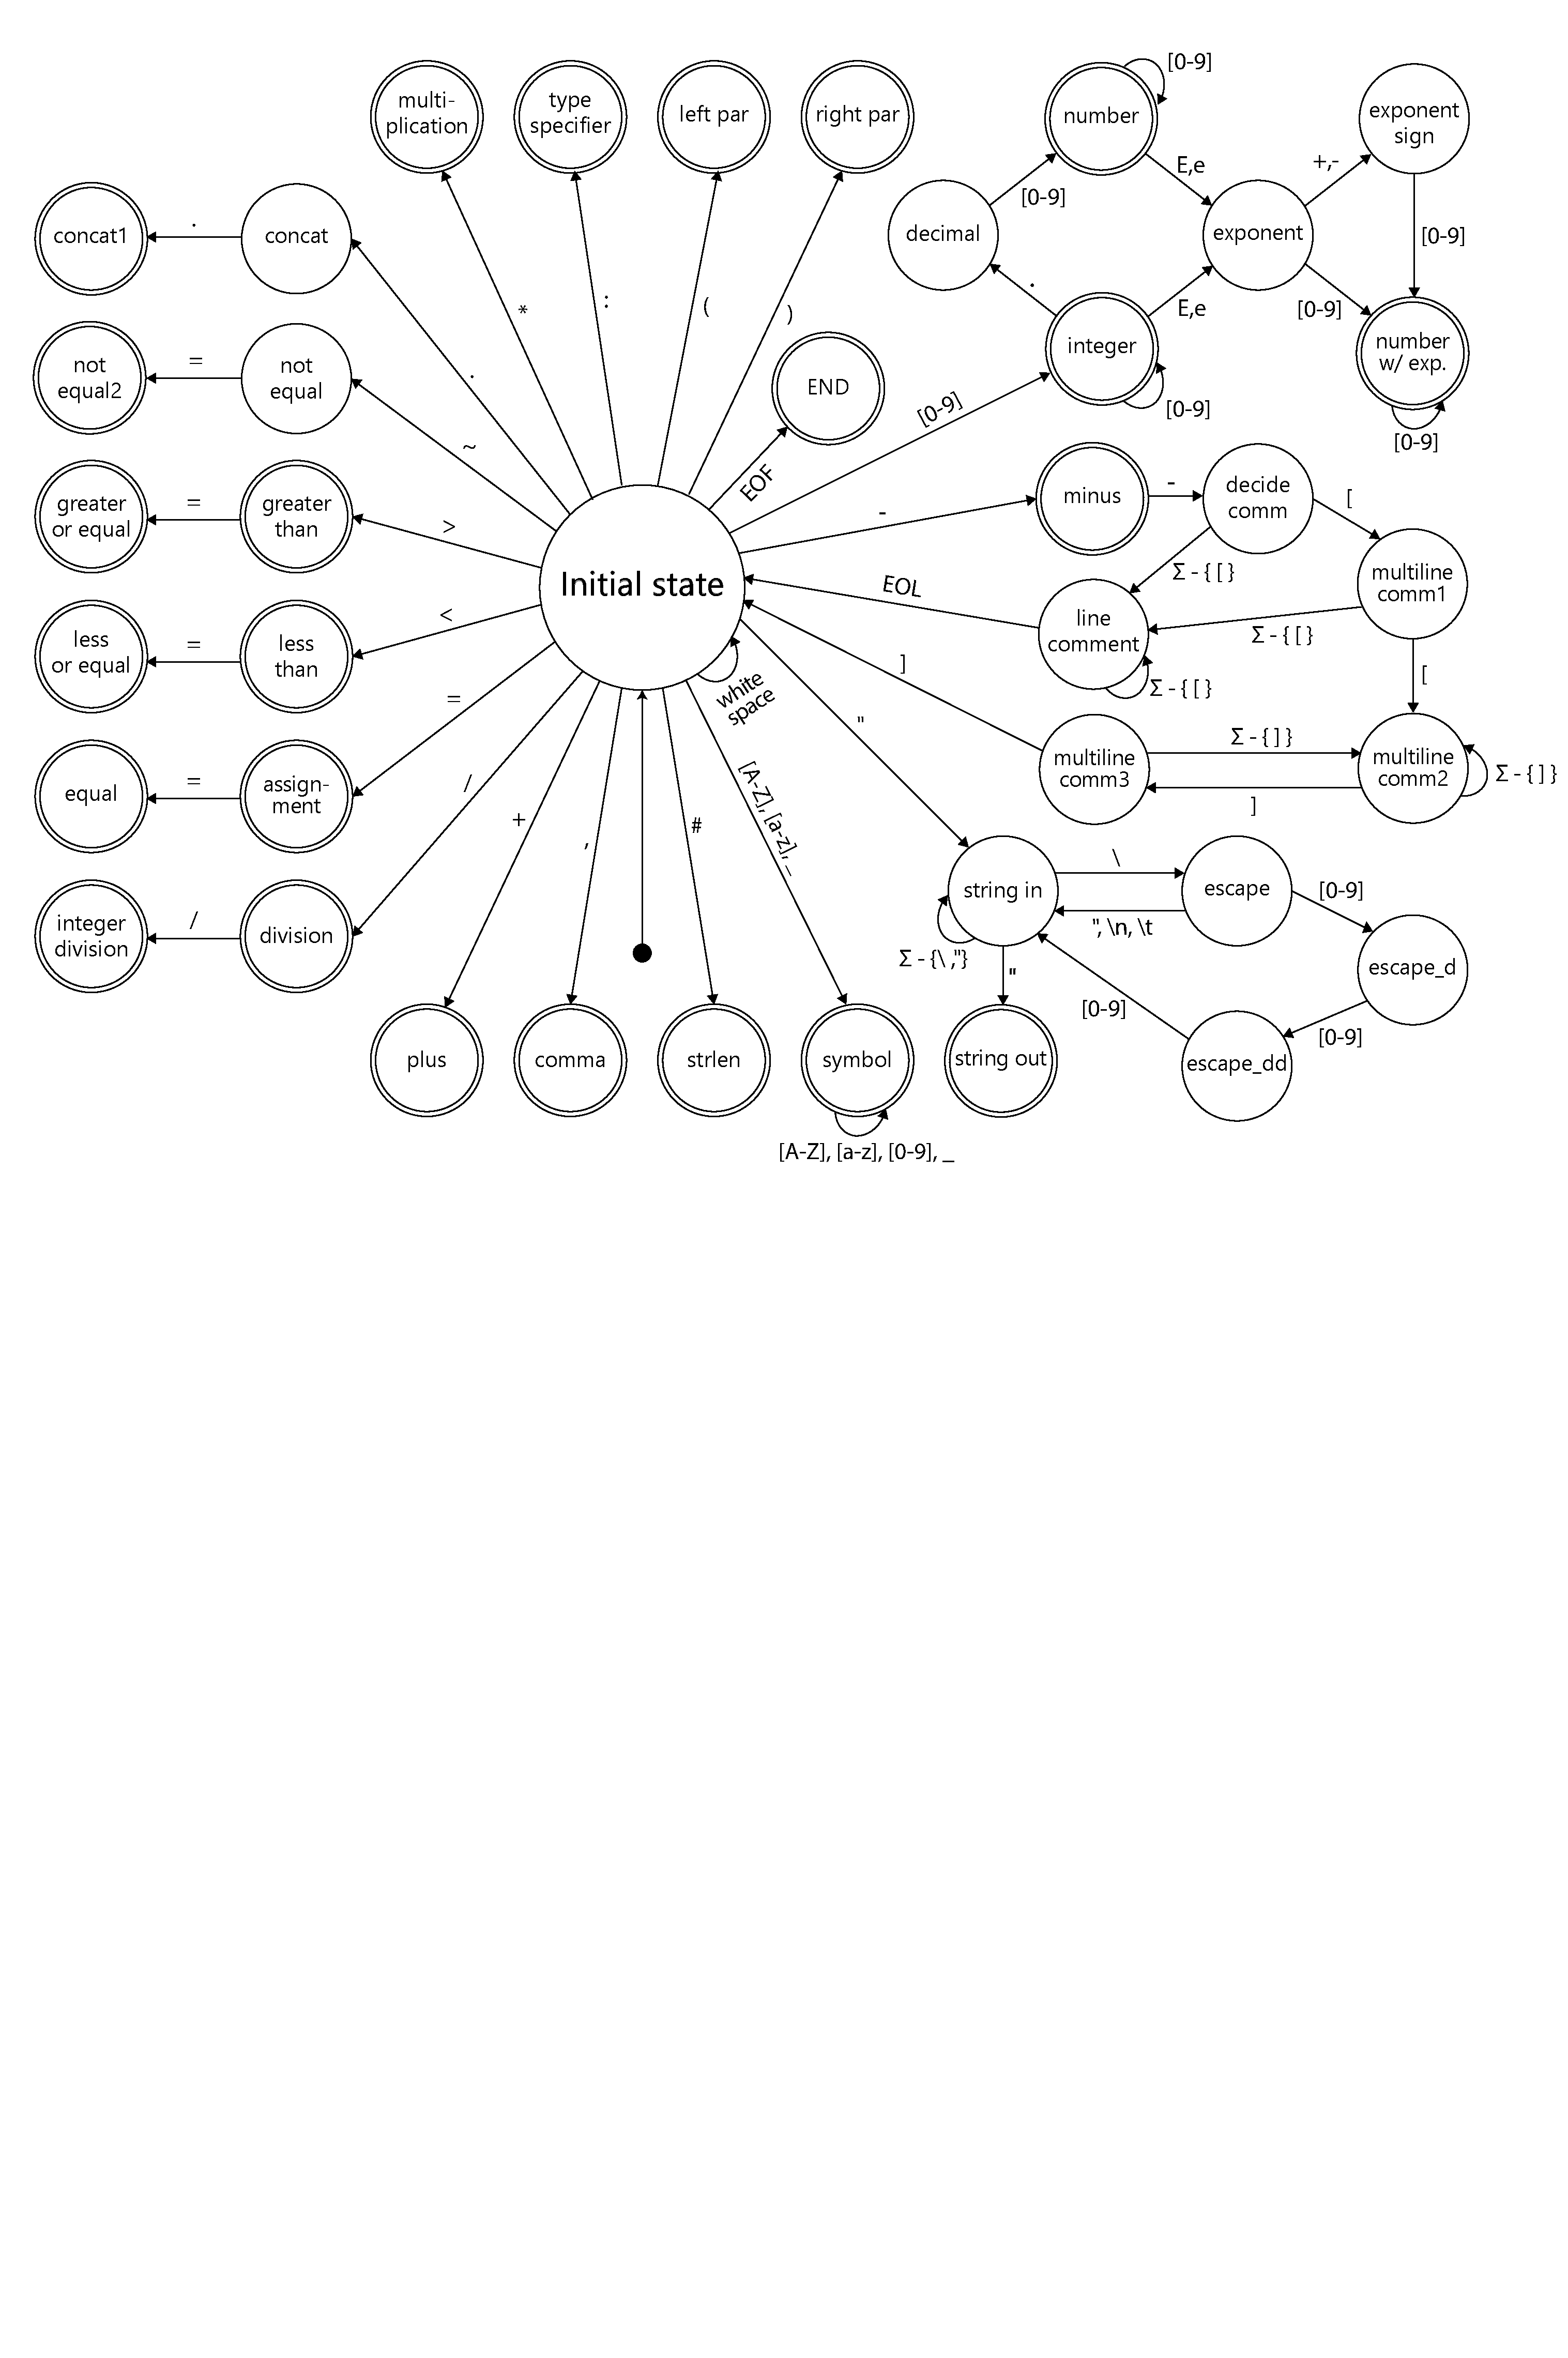
\includegraphics[scale=0.37]{images/FSM_v4.pdf}
        \end{figure}
    \subsection{Syntaktická analýza}
        \subsubsection{LL-gramatika}
        \subsubsection{LL-tabulka}
        \subsubsection{Precedenční tabulka}
    \subsection{Sémantická analýza}
    \subsection{Generátor cílového kódu}
    \subsection{Tabulka symbolů}
    \subsection{Implementovaná rozšíření}
\section{Práce v týmu}
\subsection{Rozdělení práce}
\subsection{Vývoj}
\section{Závěr}

\newpage

\section{Zdroje}
    \bibliographystyle{czechiso}
    \bibliography{references}

\end{document}
